\chapter{Supplementary Material}

\section{Periodicity, Boundaries, and the Gibbs Phenomenon}
\label{app:periodicite-bords-gibbs}

Throughout this thesis, we frequently use the discrete Fourier transform and circular
convolution. These tools implicitly rely on a signal periodization assumption. It is therefore
useful to briefly recall the relationship between periodicity, the Fourier spectrum, and boundary effects.

\begin{itemize}
    \item If a signal is defined on an infinite domain, for example $\mathbb{R}$, and is not periodic,
    its frequency content is described by a \emph{continuous spectrum}. This is the setting of the Fourier transform.

    \item If a signal is periodic, by contrast, its frequency content is \emph{discrete}:
    the signal decomposes into a sum of harmonic modes with well-defined frequencies.
    This is the setting of Fourier series.

    \item Finally, for digital signals of finite length, a periodization
    assumption is often used. The signal is then considered to be periodically extended: its two endpoints are
    artificially joined, as if the sheet on which it is drawn were rolled into a loop.
\end{itemize}

This assumption is mathematically very useful because it allows us to use the discrete Fourier
transform and to represent certain convolutions as circular convolutions. However, it can
introduce an artifact when the signal boundaries do not join naturally. If the right boundary does not meet the left boundary at a
compatible value, an artificial discontinuity appears at the junction.

This discontinuity matters from a Fourier perspective. An approximation using a finite number of Fourier modes struggles to represent an abrupt
jump. It therefore produces spurious oscillations near
the discontinuity. This behavior is known as the Gibbs phenomenon~\cite{oppenheim2009discrete}.

\begin{figure}[H]
    \centering
    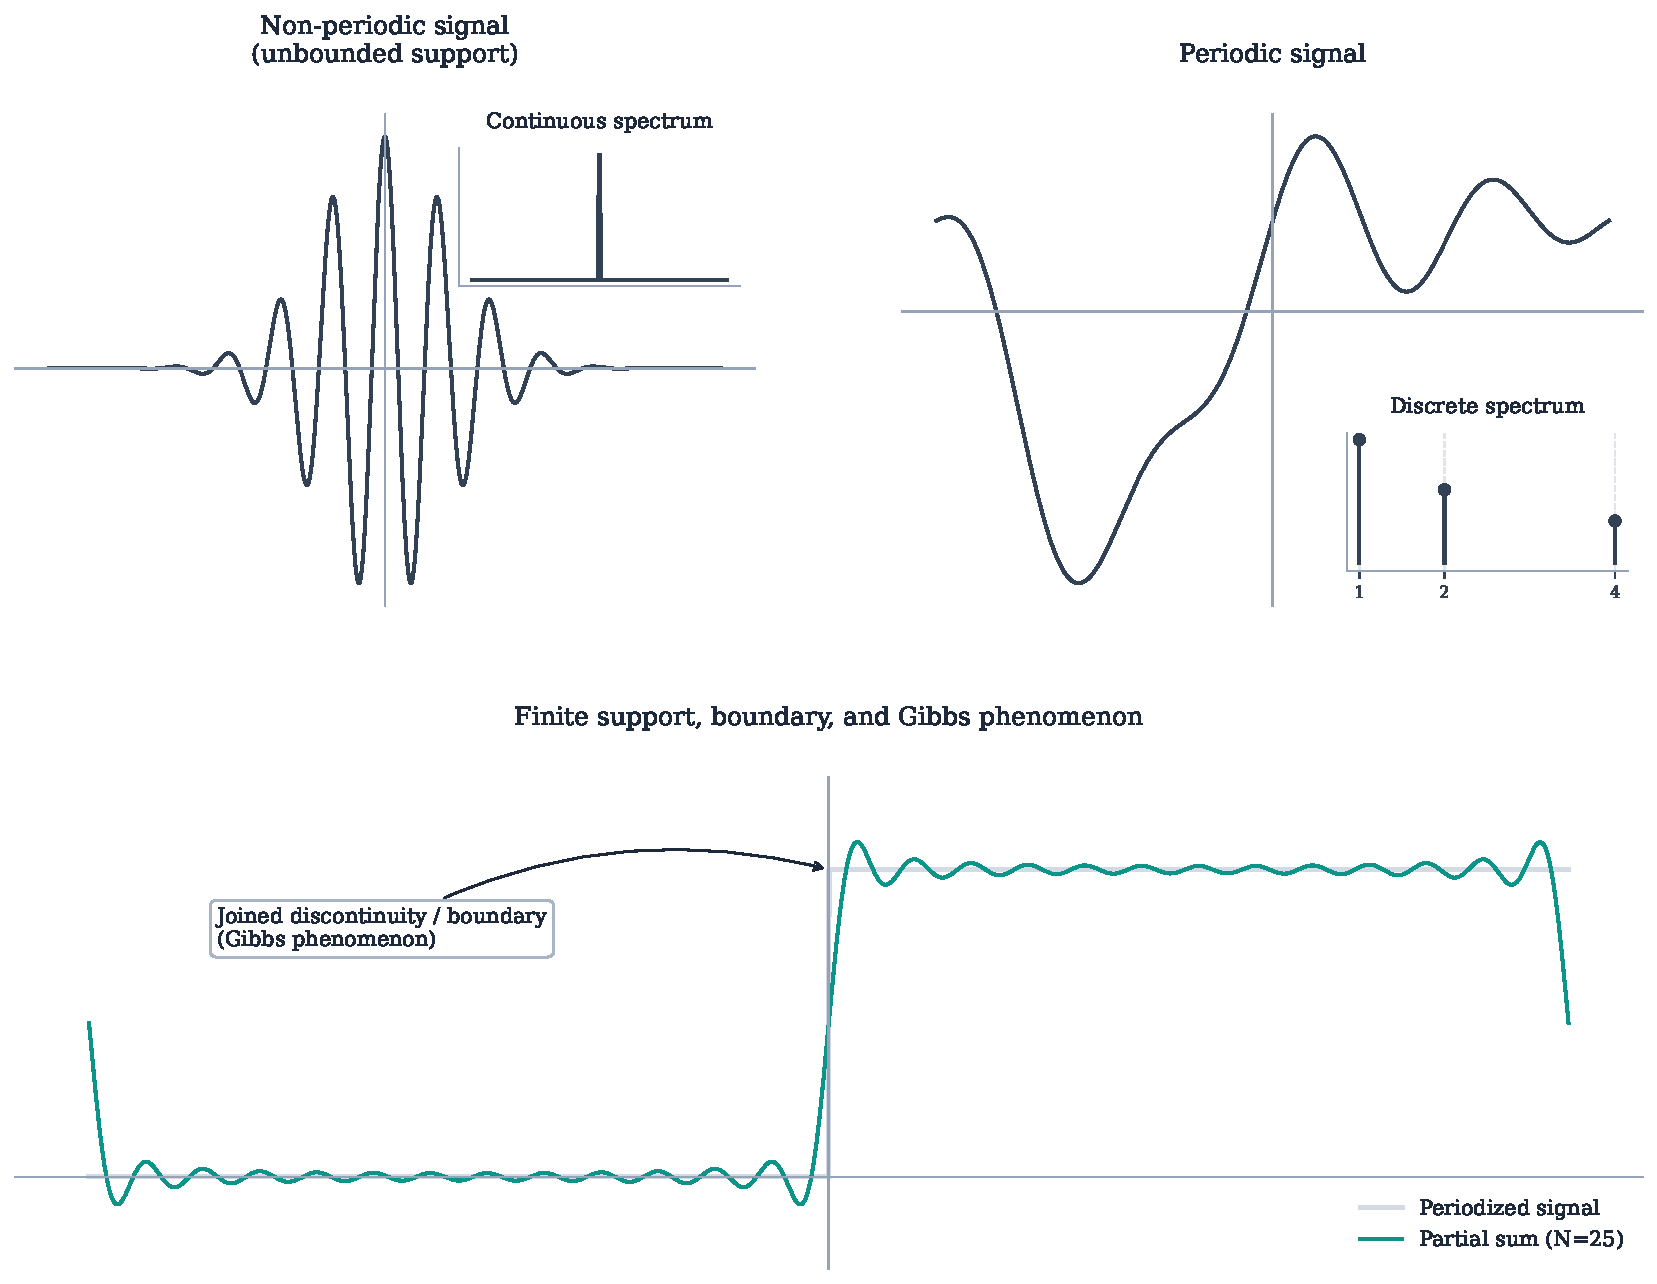
\includegraphics[width=0.8\textwidth]{figures/theory/fourier_periodicite_gibbs_en.pdf}
    \caption{Left: a nonperiodic signal defined on an infinite domain has a continuous spectrum.
    Center: a periodic signal has a discrete spectrum consisting of harmonic lines.
    Right: a signal with finite support may exhibit an artificial discontinuity when periodized.}
    \label{fig:gibbs}
\end{figure}

\section{Detailed Proof of the BCCB Structure}
\label{app:preuve_bccb}

We revisit the case of a single-channel 2D circular convolution. The goal is to show,
step by step, why the matrix $M$ associated with this convolution is block-circulant
and why each of its blocks is itself circulant.

\begin{proof}

Let $X\in\mathbb{C}^{N\times N}$ denote the input image, $Y\in\mathbb{C}^{N\times N}$ the output
image, and $h\in\mathbb{C}^{N\times N}$ the filter. Recall that, in the circular setting, 2D convolution is written as

$$\begin{aligned}
    Y[m,n] &= \sum_{a=0}^{N-1} \sum_{b=0}^{N-1} h[a,b] \, X[(m-a)\bmod N, \, (n-b)\bmod N] \\
           &= \sum_{a=0}^{N-1} \sum_{b=0}^{N-1} h[(m-a)\bmod N, \, (n-b)\bmod N] \, X[a, b].
\end{aligned}$$

With column-wise vectorization, the input entry $X[r,s]$ corresponds to the vectorized index
$r+Ns$, and the output entry $Y[m,n]$ corresponds to the vectorized index $m+Nn$. The matrix $M$ is defined
by
\[
    \operatorname{vec}(Y)=M\operatorname{vec}(X).
\]
The entry of $M$ in row $m+Nn$ and column $r+Ns$ therefore indicates how pixel
$X[r,s]$ contributes to pixel $Y[m,n]$.

According to the 2D convolution formula, this contribution is given by
\[
    M_{m+Nn,\;r+Ns}
    =
    h[(m-r)\bmod N,\,(n-s)\bmod N].
\]
This formula is central to the proof: the entry depends only on the circular
shifts between the input and output positions.

We now partition the matrix $M$ into $N\times N$ blocks, each of size $N\times N$:
\[
M =
\begin{pmatrix}
B_{0,0} & B_{0,1} & \cdots & B_{0,N-1} \\
B_{1,0} & B_{1,1} & \cdots & B_{1,N-1} \\
\vdots  & \vdots  & \ddots & \vdots \\
B_{N-1,0} & B_{N-1,1} & \cdots & B_{N-1,N-1}
\end{pmatrix}.
\]
In this partition, block $B_{n,s}$ describes the effect of column $s$ of the input image on
column $n$ of the output image.

The entries of this block are therefore
\[
    (B_{n,s})_{m,r}
    =
    M_{m+Nn,\;r+Ns}
    =
    h[(m-r)\bmod N,\,(n-s)\bmod N].
\]

Now fix two columns $n$ and $s$. Their circular shift is
\[
    \delta = (n-s)\bmod N.
\]
With this notation, the preceding expression becomes
\[
    (B_{n,s})_{m,r}
    =
    h[(m-r)\bmod N,\delta].
\]

For a fixed $\delta$, the entry $(B_{n,s})_{m,r}$ depends on $m$ and $r$ only through
the circular difference $(m-r)\bmod N$. This means that the rows of the block repeat under
circular shifts. In other words, each block $B_{n,s}$ is a circulant matrix.

To make this more explicit, define the vector
\[
h_\delta =
\begin{pmatrix}
h[0,\delta] \\
h[1,\delta] \\
\vdots \\
h[N-1,\delta]
\end{pmatrix}.
\]
Block $B_{n,s}$ is then the circulant matrix constructed from this vector:
\[
    B_{n,s}
    =
    C_{h_\delta}.
\]
Since $\delta=(n-s)\bmod N$, we can also write
\[
    B_{n,s}
    =
    C_{h_{(n-s)\bmod N}}.
\]

This formula reveals the second level of circularity. As $n$ and $s$ change,
the blocks do not vary arbitrarily: they depend only on the circular shift
$(n-s)\bmod N$. The blocks themselves are therefore arranged in a circulant pattern.

The full matrix $M$ can then be written as
\[
M =
\begin{pmatrix}
C_{h_0}     & C_{h_{N-1}} & C_{h_{N-2}} & \cdots & C_{h_1} \\
C_{h_1}     & C_{h_0}     & C_{h_{N-1}} & \cdots & C_{h_2} \\
C_{h_2}     & C_{h_1}     & C_{h_0}     & \cdots & C_{h_3} \\
\vdots      & \vdots      & \vdots      & \ddots & \vdots \\
C_{h_{N-1}} & C_{h_{N-2}} & C_{h_{N-3}} & \cdots & C_{h_0}
\end{pmatrix}.
\]

This representation clearly exhibits the two required properties:
\[
    \boxed{\text{each block is circulant}}
    \qquad\text{and}\qquad
    \boxed{\text{the blocks themselves form a circulant pattern}.}
\]
Consequently, $M$ is indeed a block-circulant matrix with circulant blocks, that is,
a BCCB matrix.

\end{proof}

\section{Detailed Proof for Skip Connections}
\label{app:preuve_skip_connection}

We revisit the identity \textit{skip connection} studied in Section~\ref{sec:skip-normalisation}.
The goal is to verify explicitly that the right singular vectors retain the same frequency structure as in the case without a \textit{skip connection}.

\begin{proof}

Let $a \in \mathbb{C}^m$ be a right singular vector of $G_{\mathrm{skip}}^{(w)}$, associated with a singular value $\sigma$ and a left singular vector $b \in \mathbb{C}^m$:
\[
G_{\mathrm{skip}}^{(w)}a = \sigma b.
\]

In the full network space, consider the vector
\[
v = a \otimes (Q_N)_w.
\]
In the same notation as before, this corresponds to
\[
v = a \otimes (F_N)_u \otimes (F_N)_v,
\]
where the flattened index $w$ corresponds to the spatial frequency pair $(u,v)$.

Now apply the operator $M_{\mathrm{skip}}$ to this vector:
\begin{align*}
M_{\mathrm{skip}}v
&=
(I_m \otimes Q_N)(L + I_{mN^2})(I_m \otimes Q_N)^H
\bigl(a \otimes (Q_N)_w\bigr).
\end{align*}

Since $(Q_N)_w = Q_N e_w$, we have
\[
a \otimes (Q_N)_w
=
(I_m \otimes Q_N)(a \otimes e_w).
\]
Thus,
\begin{align*}
M_{\mathrm{skip}}v
&=
(I_m \otimes Q_N)(L + I_{mN^2})(a \otimes e_w).
\end{align*}

The standard basis vector $e_w$ selects the coefficients associated with frequency $w$.
At this frequency, the central operator acts as the augmented mixing matrix
\[
G_{\mathrm{skip}}^{(w)} = G^{(w)} + I_m.
\]
Thus, its action on the channels separates from its action on the spatial frequency:
\begin{align*}
(L + I_{mN^2})(a \otimes e_w)
&= (G^{(w)}a + I_m a) \otimes e_w \\
&= (G_{\mathrm{skip}}^{(w)}a) \otimes e_w.
\end{align*}

Since $a$ is a right singular vector of $G_{\mathrm{skip}}^{(w)}$, we have
\[
G_{\mathrm{skip}}^{(w)}a = \sigma b.
\]
We therefore obtain
\[
(L + I_{mN^2})(a \otimes e_w) = \sigma(b \otimes e_w).
\]

Substituting this result into the expression for $M_{\mathrm{skip}}v$ gives:
\begin{align*}
M_{\mathrm{skip}}v
&=
(I_m \otimes Q_N) \bigl( \sigma(b \otimes e_w) \bigr) \\
&= \sigma \bigl( (I_m b) \otimes (Q_N e_w) \bigr) \\
&= \sigma\bigl(b \otimes (Q_N)_w\bigr).
\end{align*}

Thus, applying $M_{\mathrm{skip}}$ to the vector
\[
v = a \otimes (Q_N)_w
\]
indeed yields an output vector with the same spatial frequency:
\[
M_{\mathrm{skip}}v = \sigma\bigl(b \otimes (Q_N)_w\bigr).
\]

The spatial frequency $(Q_N)_w$ is therefore preserved. Only the overall amplitude, given by $\sigma$, and the channel profile, given by $b$, change.

Consequently, the right singular vectors of the operator with a \textit{skip connection} remain of the form
\[
a \otimes (Q_N)_w,
\]
that is,
\[
a \otimes (F_N)_u \otimes (F_N)_v.
\]
\end{proof}

\section{Graphical Representation of Stride}

\definecolor{gridblue}{HTML}{006699}
\definecolor{gridteal}{HTML}{148F77}
\definecolor{gridred}{HTML}{E74C3C}
\definecolor{selectgray}{HTML}{D3D3D3}

\begin{figure}[H]
    \centering
    \begin{tikzpicture}[scale=0.75, every node/.style={transform shape}] 

        % =========================================================================
        % GAUCHE : Stride = 1
        % =========================================================================
        \begin{scope}[shift={(0,0)}]
            % Titre parfaitement centré sur l'axe vertical de la figure (x=0)
            \node[font=\large\bfseries] at (0,6.5) {Stride = 1 (Continuous sliding)};
            
            \begin{scope}[x={(0.6cm,0.3cm)}, y={(-0.6cm,0.3cm)}, z={(0cm,0.8cm)}]
                
                % --- Image d'entrée 5x5 ---
                \fill[gridblue] (0,0,0) -- (5,0,0) -- (5,5,0) -- (0,5,0) -- cycle;
                \draw[black, thick, join=round] (0,0,0) -- (5,0,0) -- (5,5,0) -- (0,5,0) -- cycle;
                \foreach \i in {1,...,4} {
                    \draw[black, thick] (\i,0,0) -- (\i,5,0);
                    \draw[black, thick] (0,\i,0) -- (5,\i,0);
                }
                
                % --- Filtre initial ---
                \fill[gridred, opacity=0.8] (0,0,0) -- (3,0,0) -- (3,3,0) -- (0,3,0) -- cycle;
                \draw[black, thick, join=round] (0,0,0) -- (3,0,0) -- (3,3,0) -- (0,3,0) -- cycle;
                \foreach \i in {1,2} {
                    \draw[black, thick] (\i,0,0) -- (\i,3,0);
                    \draw[black, thick] (0,\i,0) -- (3,\i,0);
                }

                % --- Mouvement du filtre (Fantôme) ---
                \draw[gridred, ultra thick, dashed, opacity=1] (1,0,0) -- (4,0,0) -- (4,3,0) -- (1,3,0) -- cycle;
                
                % --- Flèche de direction unique (+1) très visible ---
                \draw[->, ultra thick, gridred, line join=round] (1.5,1.5,0) -- (2.5,1.5,0) 
                    node[midway, sloped, below, yshift=-3pt, font=\bfseries\large, fill=white, fill opacity=0.9, text opacity=1, inner sep=3pt, rounded corners=2pt] {+1};
                
                % --- Projection (Pointillés très marqués) ---
                \draw[black!70, very thick, dashed] (0,0,0) -- (1,1,4.5);
                \draw[black!70, very thick, dashed] (3,0,0) -- (2,1,4.5);
                \draw[black!70, very thick, dashed] (3,3,0) -- (2,2,4.5);
                \draw[black!70, very thick, dashed] (0,3,0) -- (1,2,4.5);
                
                % --- Image de sortie 3x3 ---
                \fill[gridteal] (1,1,4.5) -- (4,1,4.5) -- (4,4,4.5) -- (1,4,4.5) -- cycle;
                \draw[black, thick, join=round] (1,1,4.5) -- (4,1,4.5) -- (4,4,4.5) -- (1,4,4.5) -- cycle;
                \foreach \i in {2,3} {
                    \draw[black, thick] (\i,1,4.5) -- (\i,4,4.5);
                    \draw[black, thick] (1,\i,4.5) -- (4,\i,4.5);
                }
                
                \node[anchor=south east, font=\small\bfseries] at (1,4,4.7) {Output $3 \times 3$};
            
                % Pixel calculé
                \fill[selectgray, opacity=0.9] (1,1,4.5) -- (2,1,4.5) -- (2,2,4.5) -- (1,2,4.5) -- cycle;
                \draw[black, thick] (1,1,4.5) -- (2,1,4.5) -- (2,2,4.5) -- (1,2,4.5) -- cycle;
                
            \end{scope}
            
            \node[font=\small\bfseries] at (0,-1.5) {Input $5 \times 5$};
            
        \end{scope}

        % =========================================================================
        % DROITE : Stride = 2 
        % =========================================================================
        \begin{scope}[shift={(10,0)}] 
            \node[font=\large\bfseries] at (0,6.5) {Stride = 2 (Steps of 2 positions)};

            \begin{scope}[x={(0.6cm,0.3cm)}, y={(-0.6cm,0.3cm)}, z={(0cm,0.8cm)}]
                
                % --- Image d'entrée 5x5 ---
                \fill[gridblue] (0,0,0) -- (5,0,0) -- (5,5,0) -- (0,5,0) -- cycle;
                \draw[black, thick, join=round] (0,0,0) -- (5,0,0) -- (5,5,0) -- (0,5,0) -- cycle;
                \foreach \i in {1,...,4} {
                    \draw[black, thick] (\i,0,0) -- (\i,5,0);
                    \draw[black, thick] (0,\i,0) -- (5,\i,0);
                }
                
                % --- Filtre initial ---
                \fill[gridred, opacity=0.8] (0,0,0) -- (3,0,0) -- (3,3,0) -- (0,3,0) -- cycle;
                \draw[black, thick, join=round] (0,0,0) -- (3,0,0) -- (3,3,0) -- (0,3,0) -- cycle;
                \foreach \i in {1,2} {
                    \draw[black, thick] (\i,0,0) -- (\i,3,0);
                    \draw[black, thick] (0,\i,0) -- (3,\i,0);
                }

                % --- Mouvement du filtre (Fantôme) ---
                \draw[gridred, ultra thick, dashed, opacity=1] (2,0,0) -- (5,0,0) -- (5,3,0) -- (2,3,0) -- cycle;

                % --- Flèche de direction unique (+2) ---
                \draw[->, ultra thick, gridred, line join=round] (1.5,1.5,0) -- (3.5,1.5,0) 
                    node[midway, sloped, below, yshift=-3pt, font=\bfseries\large, fill=white, fill opacity=0.9, text opacity=1, inner sep=3pt, rounded corners=2pt] {+2};

                % --- Projection (Pointillés très marqués) ---
                \draw[black!70, very thick, dashed] (0,0,0) -- (1.5,1.5,4.5);
                \draw[black!70, very thick, dashed] (3,0,0) -- (2.5,1.5,4.5);
                \draw[black!70, very thick, dashed] (3,3,0) -- (2.5,2.5,4.5);
                \draw[black!70, very thick, dashed] (0,3,0) -- (1.5,2.5,4.5);
                
                % --- Image de sortie 2x2 ---
                \fill[gridteal] (1.5,1.5,4.5) -- (3.5,1.5,4.5) -- (3.5,3.5,4.5) -- (1.5,3.5,4.5) -- cycle;
                \draw[black, thick, join=round] (1.5,1.5,4.5) -- (3.5,1.5,4.5) -- (3.5,3.5,4.5) -- (1.5,3.5,4.5) -- cycle;
                \draw[black, thick] (2.5,1.5,4.5) -- (2.5,3.5,4.5);
                \draw[black, thick] (1.5,2.5,4.5) -- (3.5,2.5,4.5);
                
                \node[anchor=south east, font=\small\bfseries] at (1.5,3.5,4.7) {Output $2 \times 2$};

                % Pixel calculé
                \fill[selectgray, opacity=0.9] (1.5,1.5,4.5) -- (2.5,1.5,4.5) -- (2.5,2.5,4.5) -- (1.5,2.5,4.5) -- cycle;
                \draw[black, thick] (1.5,1.5,4.5) -- (2.5,1.5,4.5) -- (2.5,2.5,4.5) -- (1.5,2.5,4.5) -- cycle;
                
            \end{scope}
            
            \node[font=\small\bfseries] at (0,-1.5) {Input $5 \times 5$};
            
        \end{scope}

        % =========================================================================
        % LÉGENDE 
        % =========================================================================
        \node[anchor=center, draw=black!30, thick, rounded corners, fill=white, inner sep=10pt] at (5,-3.2) {
            \begin{tikzpicture}
                \fill[gridblue] (0,0) rectangle (0.5,0.5); \node[right, font=\small\bfseries] at (0.6,0.25) {Input};
                \fill[gridred, opacity=0.8] (3,0) rectangle (3.5,0.5); \node[right, font=\small\bfseries] at (3.6,0.25) {Filter};
                \fill[gridteal] (6,0) rectangle (6.5,0.5); \node[right, font=\small\bfseries] at (6.6,0.25) {Output};
                \fill[selectgray] (9,0) rectangle (9.5,0.5); \node[right, font=\small\bfseries] at (9.6,0.25) {Computed pixel};
            \end{tikzpicture}
        };

    \end{tikzpicture}
    \caption{Effect of \textit{stride} on the output spatial resolution.}
    \label{fig:stride_comparison}
\end{figure}

\section{Illustration of Average Pooling}

\begin{figure}[H]
    \centering
    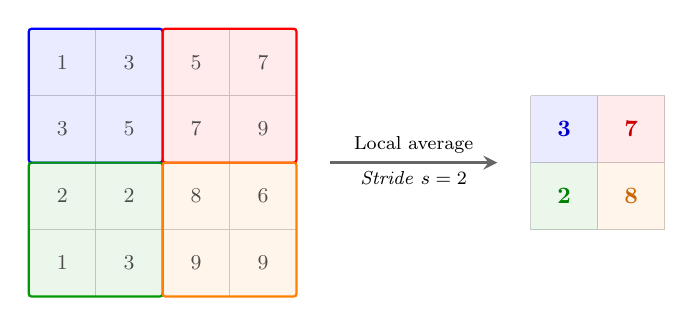
\begin{tikzpicture}[scale=0.85, transform shape]
        % --- GRILLE D'ENTREE (4x4) ---
        \draw[step=1cm, gray!40, thin] (0,0) grid (4,4);
        
        % Couleurs des blocs 2x2 (Style sobre et epure)
        \fill[blue, opacity=0.08] (0,2) rectangle (2,4);
        \fill[red, opacity=0.08] (2,2) rectangle (4,4);
        \fill[green!60!black, opacity=0.08] (0,0) rectangle (2,2);
        \fill[orange, opacity=0.08] (2,0) rectangle (4,2);

        % Cadres des blocs
        \draw[blue, thick, rounded corners=1pt] (0,2) rectangle (2,4);
        \draw[red, thick, rounded corners=1pt] (2,2) rectangle (4,4);
        \draw[green!60!black, thick, rounded corners=1pt] (0,0) rectangle (2,2);
        \draw[orange, thick, rounded corners=1pt] (2,0) rectangle (4,2);

        % Valeurs d'entree (Exemple numerique simple)
        \foreach \x/\y/\v in {0.5/3.5/1, 1.5/3.5/3, 0.5/2.5/3, 1.5/2.5/5,
                              2.5/3.5/5, 3.5/3.5/7, 2.5/2.5/7, 3.5/2.5/9,
                              0.5/1.5/2, 1.5/1.5/2, 0.5/0.5/1, 1.5/0.5/3,
                              2.5/1.5/8, 3.5/1.5/6, 2.5/0.5/9, 3.5/0.5/9} {
            \node[font=\small, text=black!70] at (\x, \y) {\v};
        }

        % --- FLECHE DE TRANSITION ---
        \draw[->, >=stealth, very thick, black!60] (4.5, 2) -- node[above, font=\footnotesize, text=black] {Local average} node[below, font=\footnotesize, text=black] {\textit{Stride} $s=2$} (7, 2);

        % --- GRILLE DE SORTIE (2x2) ---
        \begin{scope}[xshift=7.5cm, yshift=1cm]
            \draw[step=1cm, gray!40, thin] (0,0) grid (2,2);
            
            % Couleurs correspondantes
            \fill[blue, opacity=0.08] (0,1) rectangle (1,2);
            \fill[red, opacity=0.08] (1,1) rectangle (2,2);
            \fill[green!60!black, opacity=0.08] (0,0) rectangle (1,1);
            \fill[orange, opacity=0.08] (1,0) rectangle (2,1);

            % Valeurs calculees (moyennes)
            \node[font=\bfseries, text=blue!80!black] at (0.5, 1.5) {3};
            \node[font=\bfseries, text=red!80!black] at (1.5, 1.5) {7};
            \node[font=\bfseries, text=green!50!black] at (0.5, 0.5) {2};
            \node[font=\bfseries, text=orange!80!black] at (1.5, 0.5) {8};
        \end{scope}

    \end{tikzpicture}
    \caption{Spatial illustration of the \textit{average pooling} operation. Each $2 \times 2$ block of pixels in the input image is replaced by its arithmetic mean, reducing the spatial resolution by a factor of $s=2$.}
    \label{fig:avg_pooling_spatial}
\end{figure}

\section{Review of the SVD and Amplification Directions}
\label{app:svd-sensibilite}

Let
\[
    M \in \mathbb{C}^{m_{\mathrm{out}}N^2 \times m_{\mathrm{in}}N^2}
\]
be the matrix representing a multichannel convolution operator. Since this matrix is not
necessarily square, we use singular value decomposition rather than standard
eigendecomposition.

The singular value decomposition of $M$ is
\[
    M = U \Sigma V^H,
\]
where $U$ and $V$ are unitary matrices, and $\Sigma$ is a rectangular diagonal matrix
containing the singular values of $M$:
\[
    \sigma_1 \geq \sigma_2 \geq \cdots \geq 0.
\]
The columns of $V$ are called the right singular vectors of $M$: they lie in the input
space. The columns of $U$ are called the left singular vectors of $M$: they lie in
the output space.

To understand why right singular vectors describe amplification directions,
consider the positive self-adjoint matrix $M^H M$. From the SVD, we obtain
\[
    M^H M
    =
    (U\Sigma V^H)^H(U\Sigma V^H).
\]
Using $(ABC)^H = C^H B^H A^H$ gives
\[
    M^H M
    =
    V\Sigma^H U^H U \Sigma V^H.
\]
Since $U$ is unitary, $U^H U = I$, so
\[
    M^H M
    =
    V\Sigma^H \Sigma V^H.
\]
The matrix $\Sigma^H\Sigma$ is diagonal and contains the squared singular values:
\[
    \Sigma^H\Sigma
    =
    \operatorname{diag}(\sigma_1^2,\sigma_2^2,\dots).
\]
Thus,
\[
    M^H M
    =
    V
    \operatorname{diag}(\sigma_1^2,\sigma_2^2,\dots)
    V^H.
\]
This shows that the right singular vectors of $M$ are precisely the eigenvectors of
$M^H M$, and that the associated eigenvalues are the squared singular values.

In particular, if $v_i$ denotes the $i$-th column of $V$, then
\[
    M^H M v_i
    =
    V D V^H v_i
    =
    V D e_i
    =
    V(\sigma_i^2 e_i)
    =
    \sigma_i^2 v_i,
\]
where
\[
    D=\operatorname{diag}(\sigma_1^2,\sigma_2^2,\dots).
\]
Thus,
\[
    M^H M v_i = \sigma_i^2 v_i.
\]

Equivalently, the singular value $\sigma_i$ measures the amplification induced by $M$
in direction $v_i$. Indeed,
\[
    \|Mv_i\|_2^2
    =
    (Mv_i)^H(Mv_i)
    =
    v_i^H M^H M v_i
    =
    v_i^H(\sigma_i^2 v_i)
    =
    \sigma_i^2 \|v_i\|_2^2.
\]
Since $V$ is unitary, its columns form an orthonormal basis. In particular,
\[
    \|v_i\|_2 = 1.
\]
We therefore obtain
\[
    \|Mv_i\|_2 = \sigma_i.
\]

The largest singular value describes the maximum amplification of $M$ among inputs with norm
$1$:
\[
    \sigma_1
    =
    \max_{\|x\|_2=1}\|Mx\|_2.
\]
If $\sigma_1$ is simple, the direction achieving this maximum amplification is the right singular
vector $v_1$. If $\sigma_1$ has multiplicity greater than one, there is no single maximizing direction: every
unit-norm direction in the subspace associated with $\sigma_1$ yields the same amplification.

In the frequency analysis of convolutions, the network's highly sensitive directions
therefore correspond to right singular vectors associated with large singular values.

\section{Mean Fourier Spectrum of Clean Images}
\label{annexe:spectres_moyens_cifar}

This appendix presents the mean Fourier spectrum of unperturbed CIFAR-10 and CIFAR-100 images.
The aim is not to measure model sensitivity directly, but to observe which frequencies
are naturally present in the input data.

\begin{figure}[H]
    \centering
    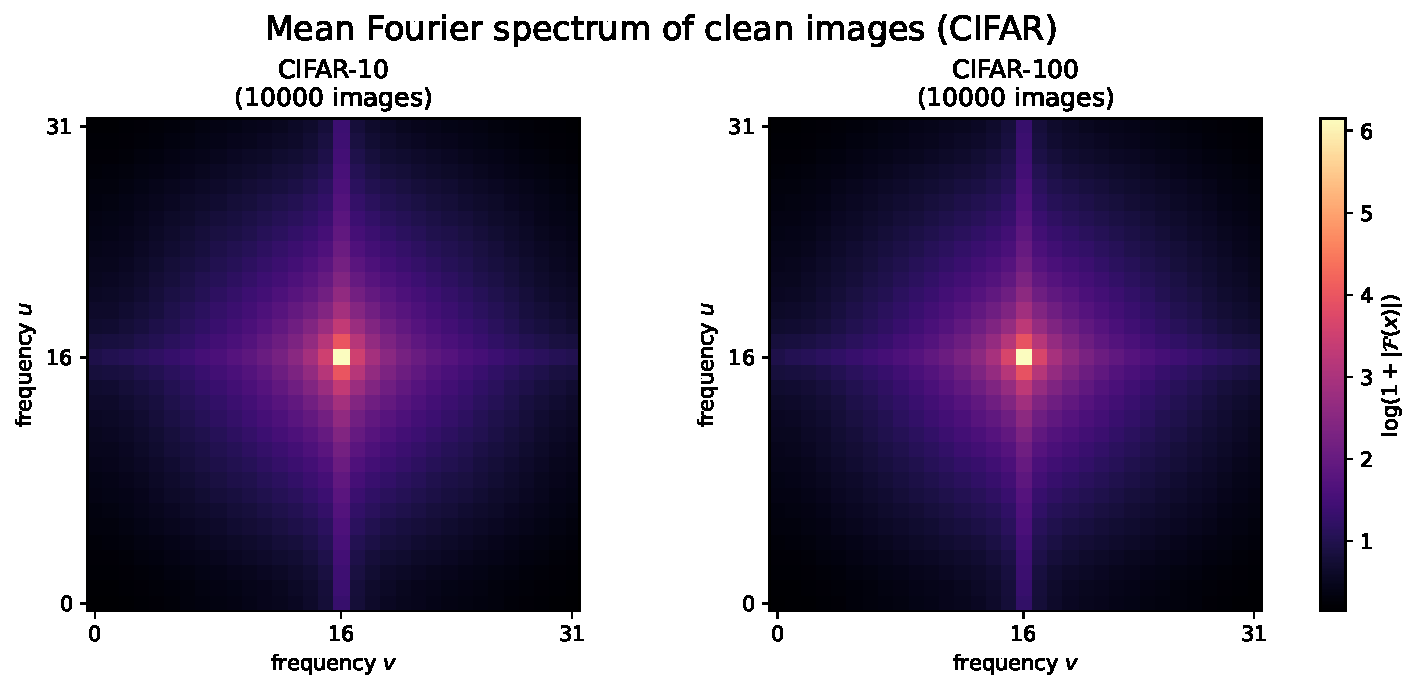
\includegraphics[width=\textwidth]{figures/results/mean_clean_spectrum_comparison_cifar_en.pdf}
    \caption{Mean Fourier spectrum of unperturbed CIFAR-10 and CIFAR-100 images. The displayed values
    correspond to $\log(1+|\mathcal{F}(x)|)$, averaged over the images in the dataset.}
    \label{fig:mean_clean_spectrum_comparison_cifar}
\end{figure}

The two datasets exhibit very similar frequency structures:
energy is strongly concentrated around the center of the spectrum and gradually decreases in an approximately
diamond-shaped pattern. The more pronounced horizontal and vertical lines also indicate that certain
frequency directions are more prevalent than others in the unperturbed images.

This observation suggests a possible interpretation of the SFA heatmaps. It shows that the input
images themselves have a nonuniform frequency organization. Model sensitivity
may therefore depend both on the architecture and on the statistics of the data used during
training.

However, this comparison remains descriptive. The mean spectrum characterizes the input images,
whereas the SFA heatmaps measure the model's response to imposed perturbations. The two should
therefore not be conflated.

\section{Supplementary Analysis: The Role of Channel Mixing in SFA}
\label{annexe:color_sfa}

In the theoretical framework presented in the previous chapter, the singular directions of a
linearized convolutional model can be written in the form
\[
    v = a \otimes q_{u,v},
\]
where \(q_{u,v}\) represents a spatial Fourier component and
\(a \in \mathbb{R}^3\) describes the mixing of the red, green, and blue channels.

The \textit{Single Fourier Attack} used in the main protocol simplifies this framework. It does not seek
to optimize the spatial frequency and the color vector \(a\) simultaneously. The same Fourier
pattern is applied to all three RGB channels, which amounts to using the vector
\[
    a_{\mathrm{uni}} = (1,1,1).
\]
The search space is therefore reduced to the choice of frequency $(u,v)$. This simplification
makes the attack much easier to evaluate, since we need only iterate over the frequencies in the
Fourier domain. It is also consistent with the $\ell_\infty$ constraint used in
the main protocol: the pattern is applied at the maximum allowed amplitude to each of the
three channels.

We then distinguish two ways of constraining channel mixing. The first
retains an $\ell_\infty$-norm constraint comparable to standard SFA, to test whether
another choice of color direction can improve the attack at the same maximum amplitude. The
second uses an $\ell_1$-type budget on the color vector's coefficients. In this case,
a vector such as $a=(3,0,0)$ is possible: the total budget is concentrated in a single channel,
which no longer corresponds exactly to the standard SFA constraint. The two variants
therefore do not measure exactly the same thing; rather, they test whether the choice of RGB
mixing can strengthen the effect of a Fourier frequency.

\subsection*{Searching for RGB Vectors at Each Frequency}

Figure~\ref{fig:color_sfa_foolratio_and_activation_grids} compares standard SFA with variants
in which the RGB vector \(a\) is chosen from a limited set of possible combinations.

\begin{figure}[H]
    \centering
    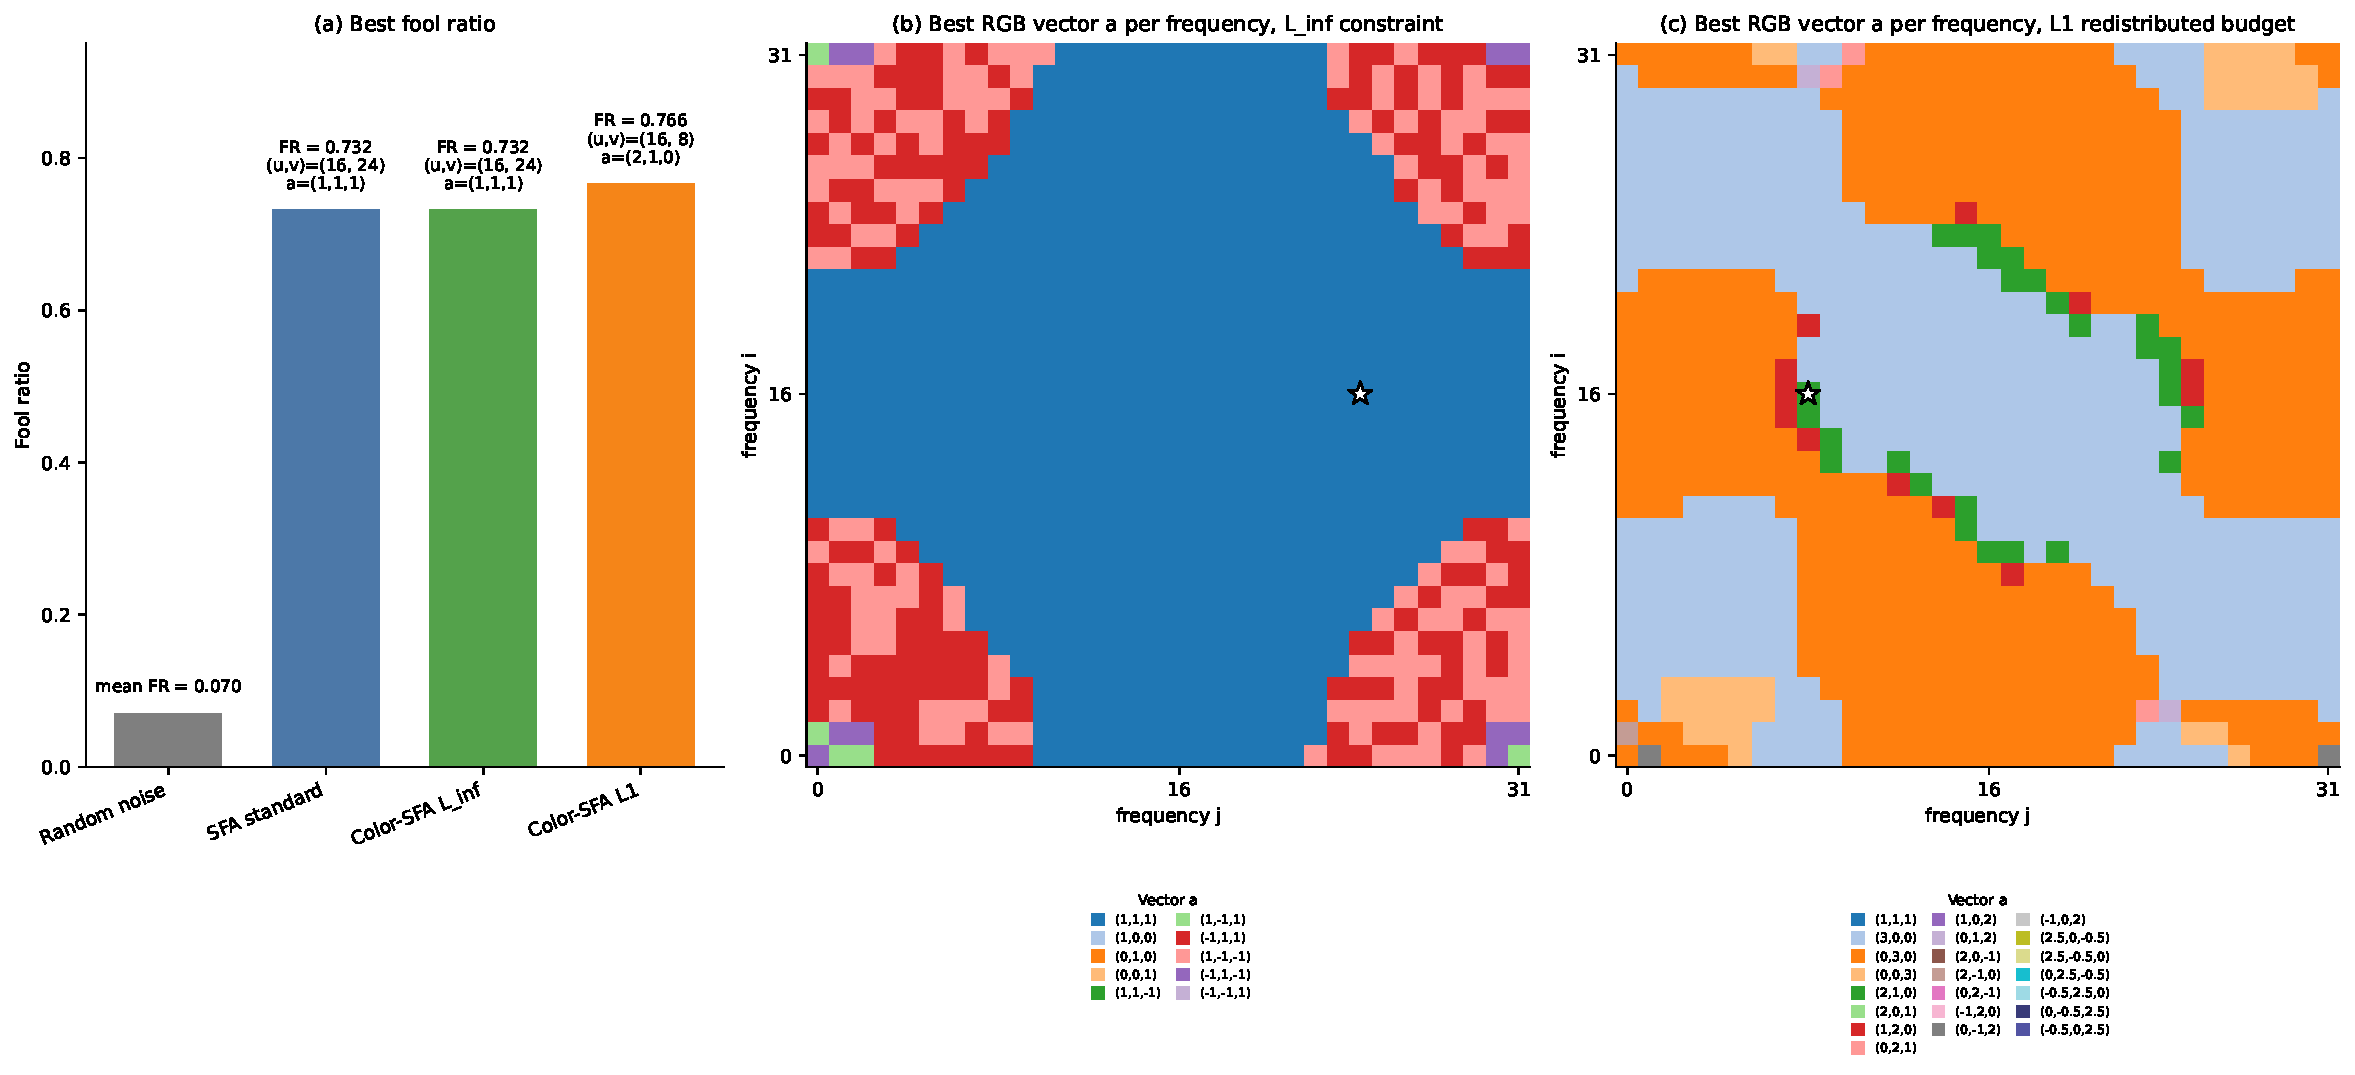
\includegraphics[width=\textwidth]{figures/results/color_sfa_foolratio_and_activation_grids.pdf}
    \caption{Comparison between standard SFA and variants in which the RGB vector \(a\) is chosen for each frequency.
    Left: the best \textit{fool ratio} obtained by each method is compared with the random-noise
    baseline. Center and right: each cell indicates the best RGB vector found for the corresponding
    frequency under two different budget constraints.}
    \label{fig:color_sfa_foolratio_and_activation_grids}
\end{figure}

In the variant renormalized in the $\ell_\infty$ norm, the best color variant achieves
almost the same result as standard SFA. This indicates that, under this constraint,
choosing a different RGB mixture does not significantly improve the attack compared with the
uniform direction $(1,1,1)$.

With the variant using an $\ell_1$ budget on the color coefficients, the best score increases slightly,
from approximately \(0.732\) to \(0.766\), with frequency \((16,8)\) and vector \(a=(2,1,0)\).
This improvement is fairly modest in our case.

\subsection*{Comparison of Fixed Color Directions}

We then compared several simple color directions:
\[
(1,1,1), \quad (1,0,0), \quad (0,1,0), \quad (0,0,1),
\]
as well as opponent color directions:
\[
(1,-1,0), \quad (1,0,-1), \quad (0,1,-1),
\]
and a luminance-like direction.

The results in Figure~\ref{fig:color_sfa_cifar10} show that the standard direction
$(1,1,1)$ remains by far the most effective. Directions applied to a single channel have a
weaker effect, while the opponent color directions $(1,-1,0)$, $(1,0,-1)$, and
$(0,1,-1)$ yield almost zero fool ratios.

\begin{figure}[H]
    \centering
    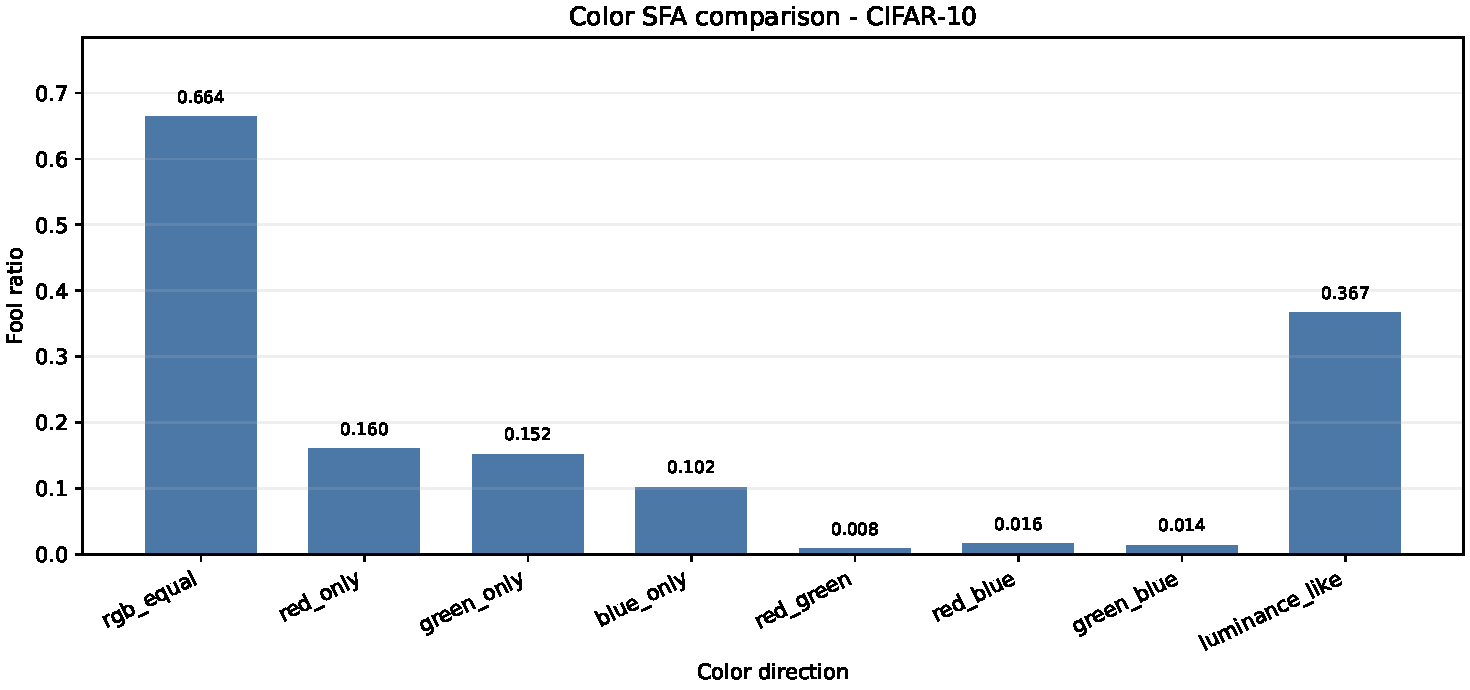
\includegraphics[width=0.85\textwidth]{figures/results/color_sfa_cifar10_barplot.pdf}
    \caption{Comparison of several color directions for the \textit{Single Fourier Attack}
    on CIFAR-10.}
    \label{fig:color_sfa_cifar10}
\end{figure}

This observation suggests that, for the frequency studied, opponent color directions
are weakly transmitted by the network. We can interpret this using the multichannel
framework. For a fixed frequency $(u,v)$, the effect of a color direction
$a \in \mathbb{R}^3$ is described by the mixing matrix $G^{(u,v)}$:
\[
    \beta = G^{(u,v)}a.
\]
Standard SFA corresponds to the choice
\[
    a_{\mathrm{uni}} = (1,1,1),
\]
that is, a common variation in all three RGB channels.

\paragraph{Ideally symmetric case.}
Suppose that, at the frequency considered, the network responds identically to the three
input channels. This amounts to assuming that the three columns of $G^{(u,v)}$ are identical:
\[
    G^{(u,v)}
    =
    \begin{pmatrix}
    | & | & | \\
    g & g & g \\
    | & | & |
    \end{pmatrix}
    =
    g
    \begin{pmatrix}
    1 & 1 & 1
    \end{pmatrix},
\]
where $g \in \mathbb{C}^{m_{\mathrm{out}}}$ describes the network's common frequency response.

Then, for any color direction $a=(a_R,a_G,a_B)$, we obtain
\[
    G^{(u,v)}a
    =
    g(a_R+a_G+a_B).
\]
Amplification therefore depends only on the sum of the components of $a$. Under an
$\ell_\infty$ constraint comparable to that of standard SFA,
\[
    |a_R|, |a_G|, |a_B| \leq 1,
\]
the absolute value of this sum is maximized by
\[
    a=(1,1,1)
\]
or its negative. Thus, in this simplified symmetric setting, the uniform direction
$a_{\mathrm{uni}}$ is optimal.

Conversely, any color direction satisfying
\[
    a_R+a_G+a_B=0
\]
is annihilated by $G^{(u,v)}$. This is the case for the opponent color directions
\[
    (1,-1,0), \qquad (1,0,-1), \qquad (0,1,-1).
\]
In this simplified model, these directions therefore belong to the kernel of the per-frequency
mixing matrix:
\[
    G^{(u,v)}a = 0.
\]

\paragraph{Approximately symmetric case.}
In a real network, the columns of $G^{(u,v)}$ are not exactly identical. However, we can
separate a component common to all three channels from a residual term:
\[
    G^{(u,v)}
    =
    g
    \begin{pmatrix}
    1 & 1 & 1
    \end{pmatrix}
    + E,
\]
where we can take
\[
    g
    =
    \frac{1}{3}G^{(u,v)}
    \begin{pmatrix}
    1 \\ 1 \\ 1
    \end{pmatrix}.
\]
The term $E$ then measures the deviation from a response that is perfectly shared by all three channels.

For an opponent color direction such that $a_R+a_G+a_B=0$, the common component
vanishes:
\[
    G^{(u,v)}a = Ea.
\]
Thus, if $\|E\|$ is small, then
\[
    \|G^{(u,v)}a\|_2
    \leq
    \|E\|\,\|a\|_2.
\]
Opponent color directions are therefore no longer exactly annihilated, but they remain
weakly transmitted when frequency-dependent channel mixing is close to a common
response.

This proposition provides a theoretical interpretation of the results observed in
Figure~\ref{fig:color_sfa_cifar10}. The high effectiveness of $(1,1,1)$ suggests that the frequency
studied primarily activates a direction common to the channels, while the low scores
of opponent color directions may be explained by near cancellation in
frequency-dependent channel mixing.

\section{Internal Heatmaps by Layer}
\label{annexe:heatmaps_internes_couches}

To complement the amplification analysis presented in the main chapter, we visualize here
the effect of Fourier perturbations at different internal levels of the network. For each frequency,
we measure the normalized mean change in activations after perturbation and then
compare it with the final \textit{fool ratio}.

\begin{figure}[H]
    \centering
    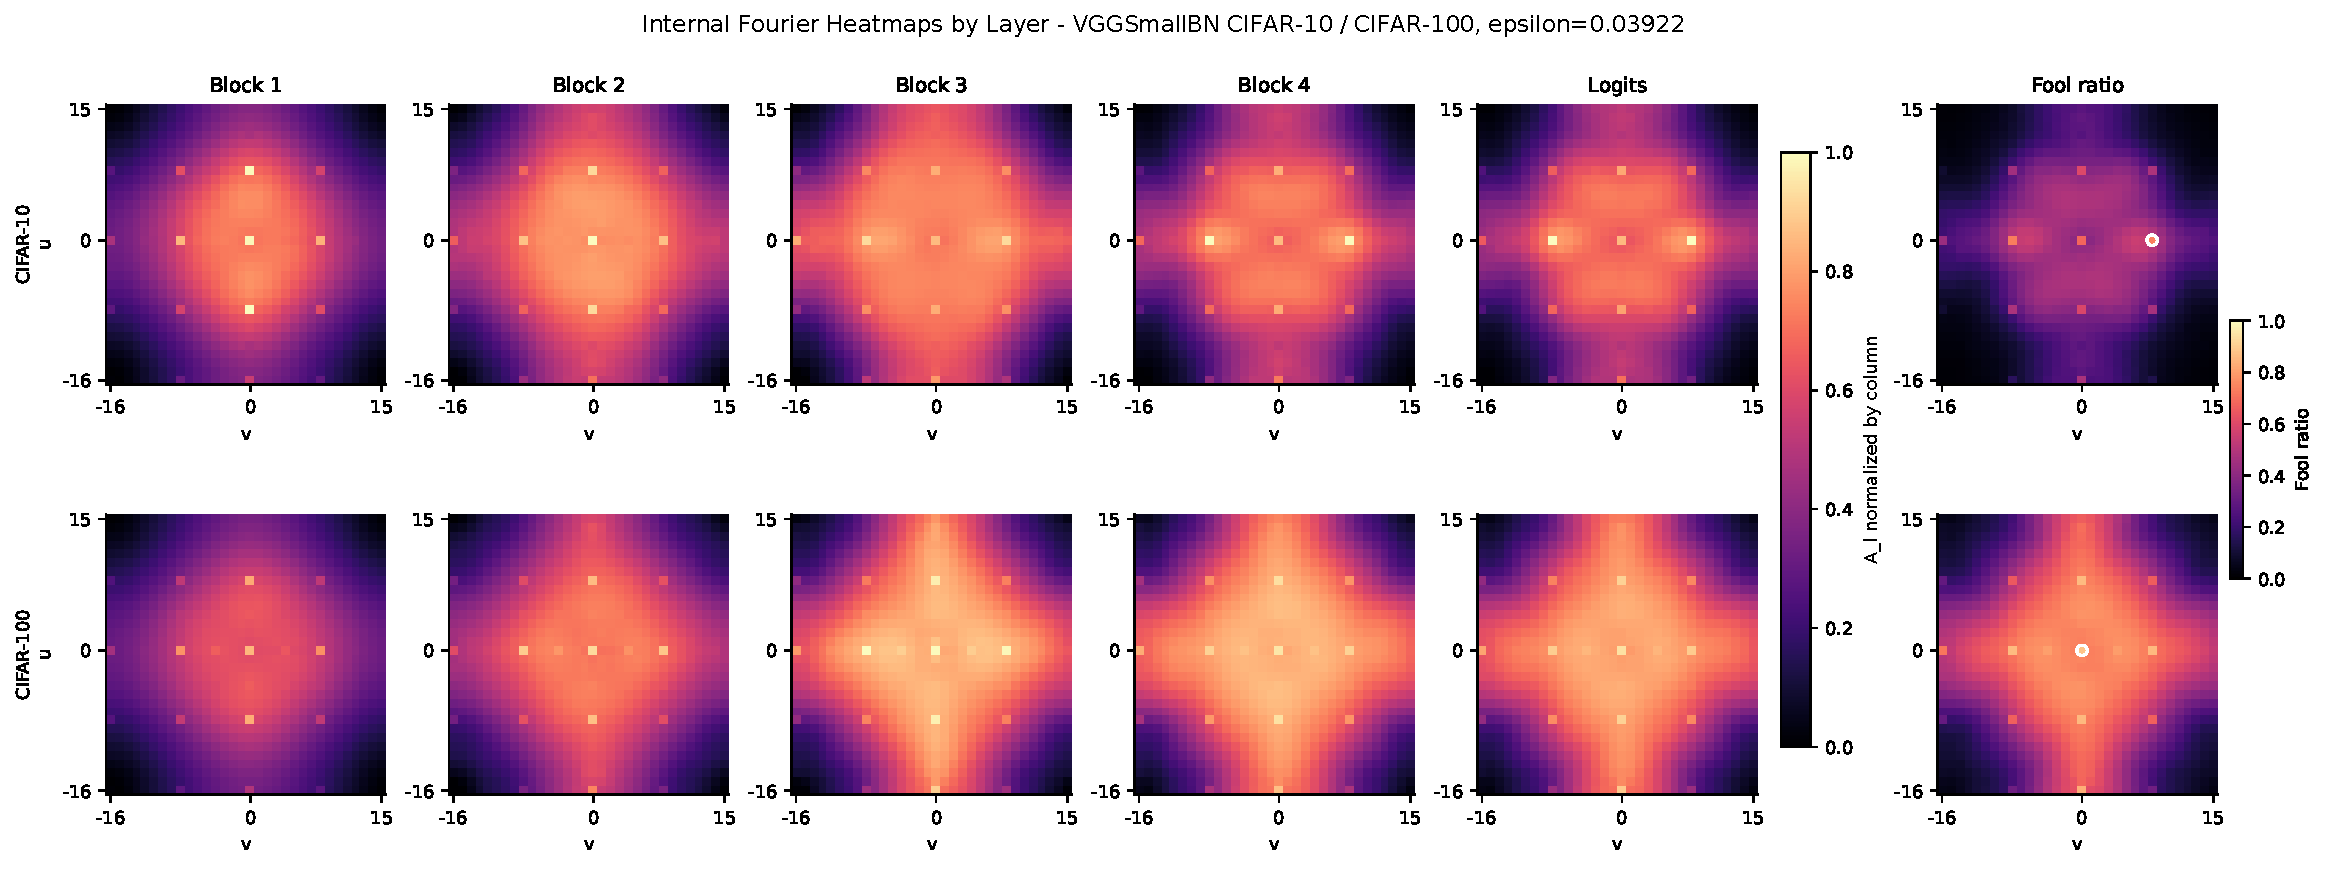
\includegraphics[width=\textwidth]{figures/results/layerwise_fourier_heatmaps_comparison_vgg_cifar10_cifar100_en.pdf}
    \caption{Internal heatmaps by layer for \texttt{VGGSmallBN} on CIFAR-10 and CIFAR-100.
    The first columns show the normalized mean change in internal activations after
    Fourier perturbation. The last column shows the final \textit{fool ratio}.}
    \label{fig:annexe_layerwise_fourier_heatmaps}
\end{figure}

These visualizations show that the frequency structure observed in the final heatmaps is
already present in the network's internal representations. It becomes more pronounced in deeper blocks and
in the logits, suggesting that certain frequencies are progressively amplified during
convolutional processing.

\section{Further Analysis of Logit Margins and Local Boundaries}
\label{annexe:marges-logits}

This appendix complements the experimental analysis in Chapter~4. The goal is to better understand
why the model trained on CIFAR-100 appears more fragile than the one trained on CIFAR-10.

\subsection{Distribution of Logit Margins}

For each image in the test set, we compute the logits produced by the model. Let
$z_{(1)}$ denote the largest logit and $z_{(2)}$ the second-largest logit. The logit margin is defined as
\[
    m(x) = z_{(1)}(x) - z_{(2)}(x).
\]

This quantity simply measures the gap between the predicted class and its closest competing class according to
the model.

Figure~\ref{fig:logit-margin-histograms} compares the distributions of logit margins for
VGGSmallBN on CIFAR-10 and CIFAR-100. The CIFAR-100 distribution is
much more concentrated at small margins. The median is approximately $4.15$ for CIFAR-100,
compared with approximately $11.12$ for CIFAR-10. This means that, on CIFAR-100, the model's predictions
are, on average, less strongly separated from their second-best class.

\begin{figure}[H]
    \centering
    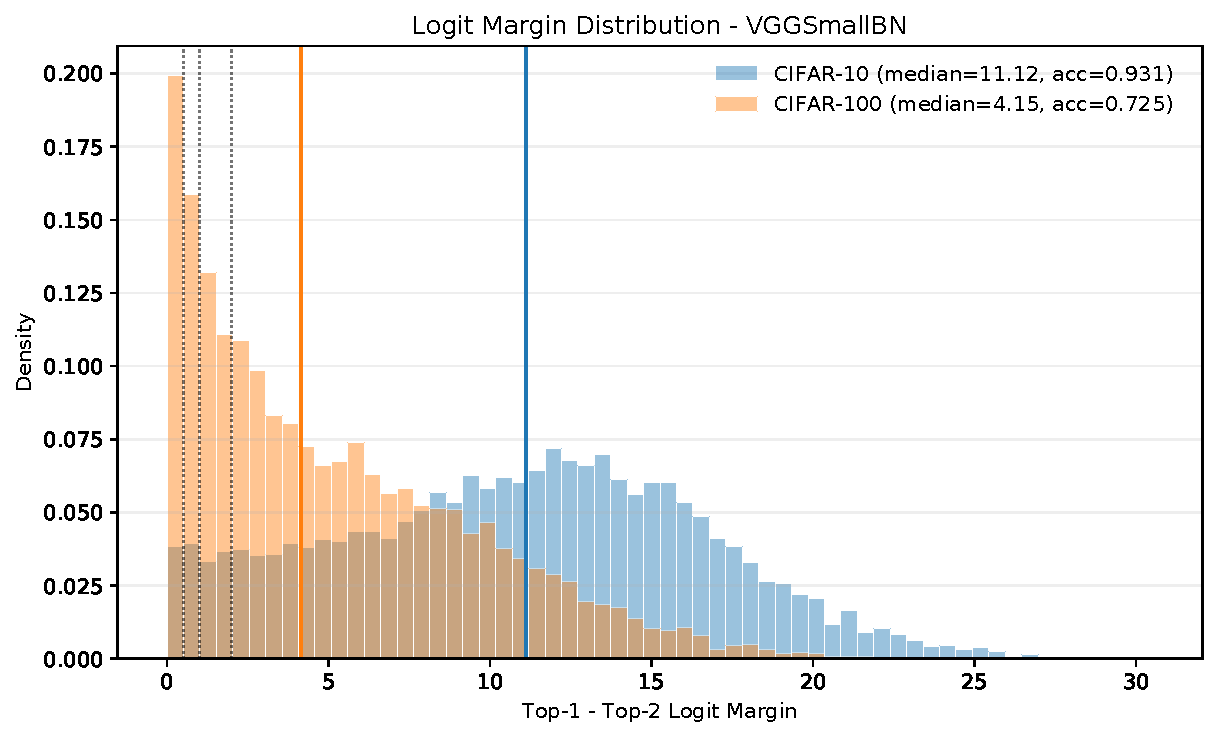
\includegraphics[width=0.85\textwidth]{figures/results/logit_margin_histograms_cifar10_cifar100_en.pdf}
    \caption{Distribution of logit margins for VGGSmallBN on CIFAR-10 and CIFAR-100. The margin is defined as the difference between the largest and second-largest logits.}
    \label{fig:logit-margin-histograms}
\end{figure}

This result provides further support for the interpretation proposed in Chapter~4:
the greater fragility observed on CIFAR-100 arises not only from the choice of a particular
frequency, but also from the apparently weaker separation between the model's decisions.

% \subsection{Carte moyenne de stabilité locale}

% En complément de l'analyse des marges logits, nous construisons une carte moyenne de stabilité
% locale autour des images correctement classées. L'objectif est de visualiser, dans une coupe
% bidimensionnelle de l'espace d'entrée, dans quelle mesure les prédictions restent stables lorsque
% l'on perturbe les images selon deux directions fréquentielles sensibles.

% Pour une image $x$, on considère les perturbations de la forme
% \[
%     x_{\alpha,\beta}
%     =
%     x + \alpha d_1 + \beta d_2,
% \]
% où $d_1$ correspond à la direction SFA principale du dataset, et $d_2$ à une seconde direction
% fréquentielle sensible.

% Pour chaque point $(\alpha,\beta)$ de la grille, nous calculons la proportion d'images pour
% lesquelles la prédiction reste identique à celle de l'image propre :
% \[
%     P_{\mathrm{same}}(\alpha,\beta)
%     =
%     \frac{1}{M}
%     \sum_{k=1}^{M}
%     \mathbf{1}\left[
%         f(x_k+\alpha d_1+\beta d_2)=f(x_k)
%     \right].
% \]
% Cette quantité vaut $1$ lorsque toutes les images gardent la même prédiction, et $0$ lorsque
% toutes les prédictions changent. Elle fournit donc une mesure moyenne de la stabilité locale du
% modèle dans la coupe considérée.

% Les cartes sont calculées sur $500$ images correctement classées par dataset, avec une grille
% de taille $41\times 41$.

% \begin{figure}[H]
%     \centering
%     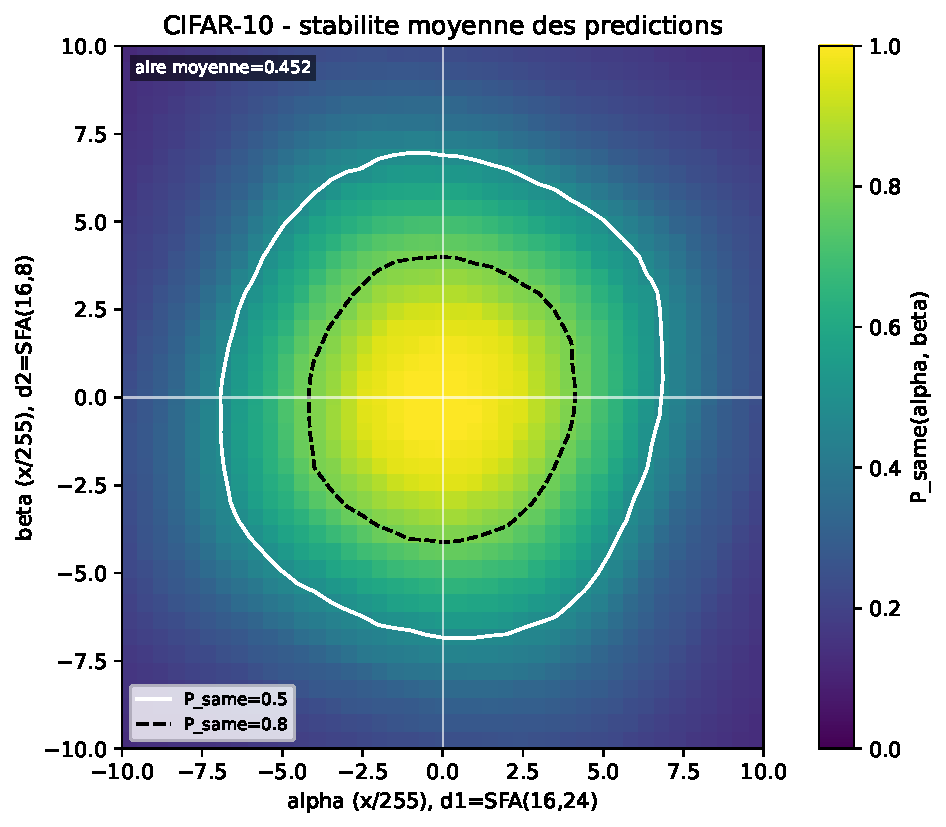
\includegraphics[width=0.48\textwidth]{figures/results/average_decision_boundary_cifar10.pdf}
%     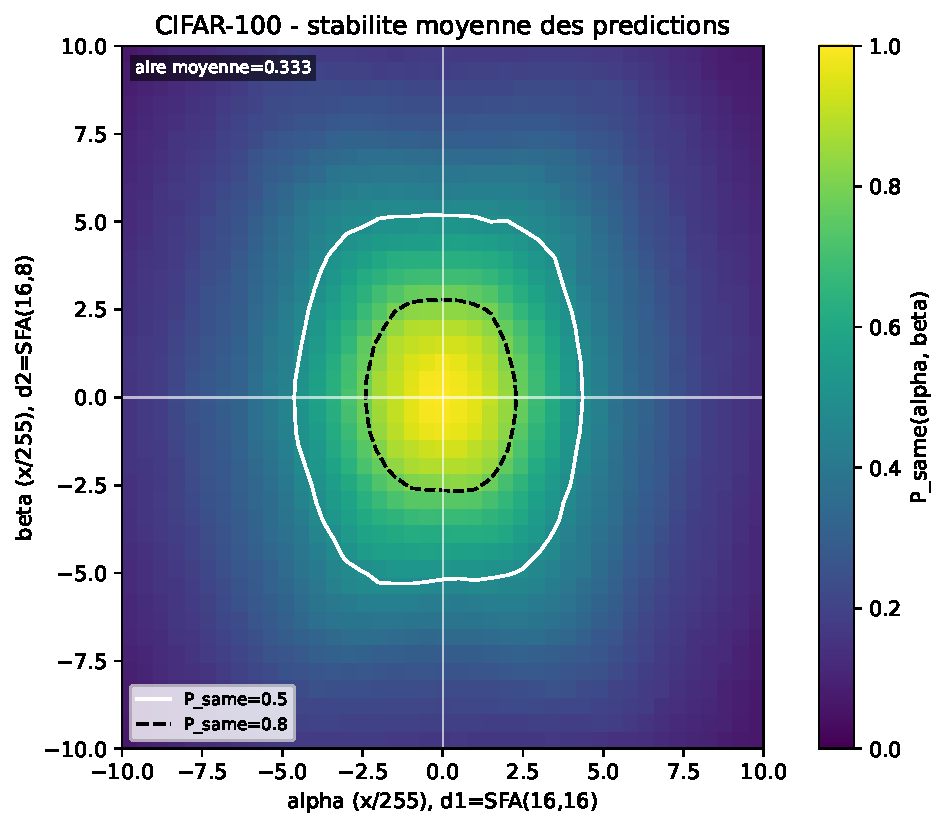
\includegraphics[width=0.48\textwidth]{figures/results/average_decision_boundary_cifar100.pdf}
%     \caption{Cartes moyennes de stabilité locale pour VGGSmallBN sur CIFAR-10 et CIFAR-100. Chaque point indique la proportion d'images dont la prédiction reste inchangée après perturbation selon deux directions fréquentielles sensibles.}
%     \label{fig:average-decision-boundary}
% \end{figure}

% \begin{table}[H]
%     \centering
%     \begin{tabular}{lcccc}
%         \toprule
%         Dataset & Aire stable moyenne & Largeur $P_{\mathrm{same}}\geq 0.5$ & Largeur $P_{\mathrm{same}}\geq 0.8$ & $\alpha$ critique moyen \\
%         \midrule
%         CIFAR-10  & 0.4518 & $13.00/255$ & $8.00/255$ & $5.81/255$ \\
%         CIFAR-100 & 0.3330 & $8.50/255$  & $4.00/255$ & $4.46/255$ \\
%         \bottomrule
%     \end{tabular}
%     \caption{ Les largeurs sont mesurées sur la ligne $\beta=0$, avec Les coefficients $\alpha$ et 
%     $\beta$ qui varient dans l'intervalle $[-10/255,10/255]$}
%     \label{tab:average-decision-boundary}
% \end{table}

% Les résultats du tableau~\ref{tab:average-decision-boundary} montrent que la région moyenne de
% stabilité est plus réduite sur CIFAR-100 que sur CIFAR-10. L'aire stable moyenne passe de
% $0.4518$ à $0.3330$, et la largeur de la région stable le long de la direction SFA diminue également.
% Pour le seuil $P_{\mathrm{same}}\geq 0.8$, cette largeur est divisée par deux, passant de $8.00/255$
% sur CIFAR-10 à $4.00/255$ sur CIFAR-100.

% Cette observation est cohérente avec les résultats principaux du chapitre~4 : le modèle entraîné
% sur CIFAR-100 est globalement plus sensible aux perturbations fréquentielles. Elle complète
% également l'analyse des marges logits, en montrant que cette fragilité se manifeste aussi dans
% une coupe locale de l'espace d'entrée.

% Il faut toutefois rester prudent dans l'interprétation. Ces cartes ne représentent pas la frontière
% de décision complète du réseau, qui vit dans un espace de dimension $32\times32\times3$.
% Elles décrivent seulement une coupe bidimensionnelle construite à partir de deux directions
% fréquentielles sensibles. Elles doivent donc être lues comme une visualisation complémentaire,
% et non comme une preuve complète de la géométrie globale des frontières de décision.
